\documentclass{article}
\usepackage[paperwidth=22cm,paperheight=9cm,margin=0cm,noheadfoot]{geometry}
\usepackage{amsmath,amssymb}
\usepackage{tikz}
\usetikzlibrary{arrows.meta,positioning,calc,backgrounds}
\usepackage{xcolor}
\usepackage[T1]{fontenc}
\usepackage{lmodern}
\usepackage{tgheros}
\usepackage{sansmath}
\renewcommand{\familydefault}{\sfdefault}
\sansmath
\pagestyle{empty}
\setlength{\parindent}{0pt}

% === Colors ===
\definecolor{deepblue}{HTML}{1A5276}
\definecolor{midblue}{HTML}{2980B9}
\definecolor{lightblue}{HTML}{D4E6F1}

\definecolor{deeporange}{HTML}{B9470B}
\definecolor{midorange}{HTML}{E67E22}
\definecolor{lightorange}{HTML}{FDEBD0}

\definecolor{deeppurple}{HTML}{6C3483}
\definecolor{midpurple}{HTML}{8E44AD}
\definecolor{lightpurple}{HTML}{E8DAEF}

\definecolor{deepgray}{HTML}{2C3E50}
\definecolor{midgray}{HTML}{7F8C8D}
\definecolor{panelbg}{HTML}{FAFCFE}

\begin{document}
\vspace*{0pt}\noindent
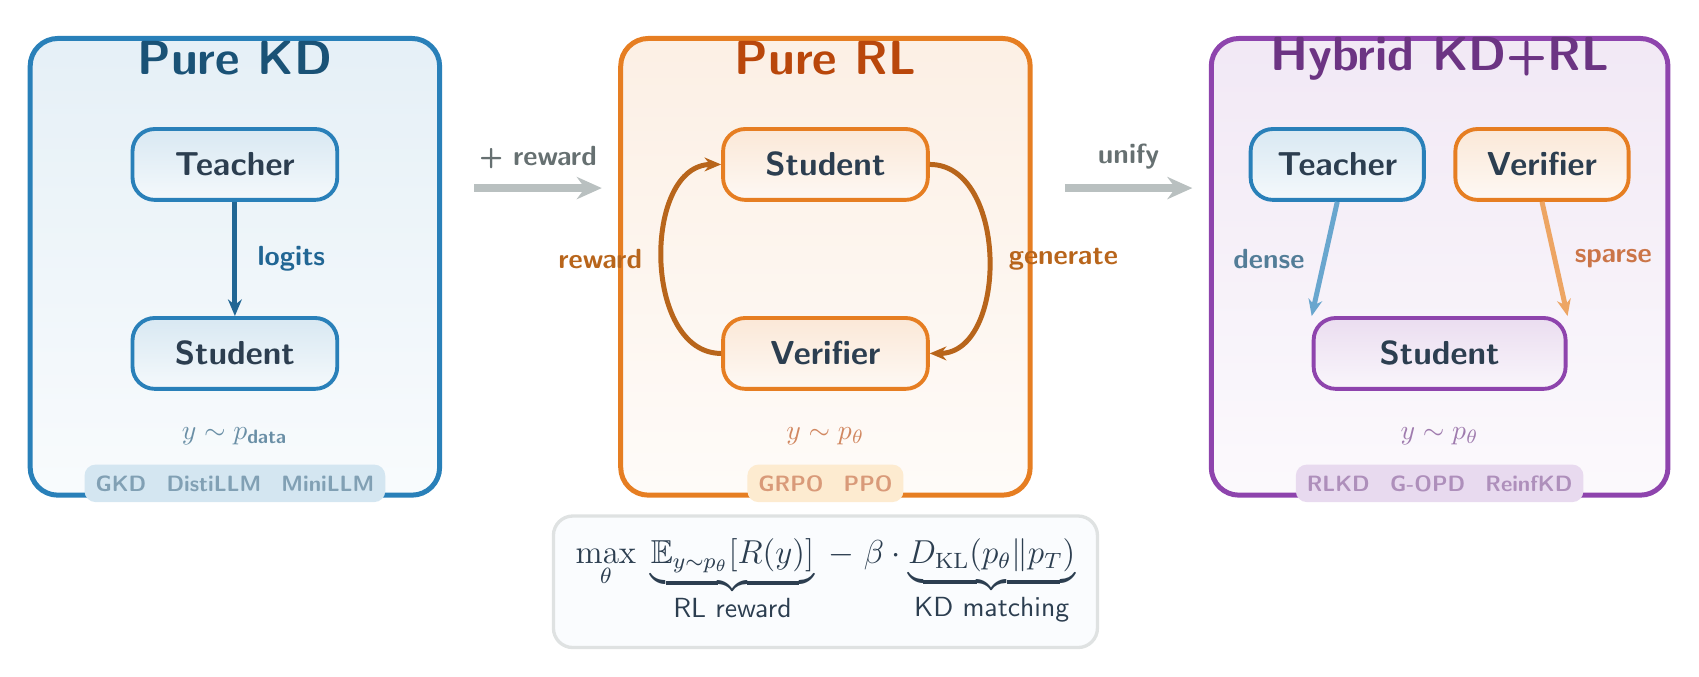
\begin{tikzpicture}[
    >=Stealth,
    stagebox/.style={
      draw=#1, line width=1.8pt, rounded corners=10pt,
      top color=#1!12, bottom color=#1!3,
      minimum width=5.2cm, minimum height=5.8cm,
      inner sep=0pt,
    },
    entity/.style={
      draw=#1, line width=1.4pt, rounded corners=8pt,
      top color=#1!18, bottom color=#1!5,
      font=\large\bfseries, text=deepgray,
      minimum width=2.6cm, minimum height=0.9cm,
      text centered, inner sep=5pt,
    },
    evolve/.style={
      -{Stealth[length=9pt,width=8pt]}, line width=3pt, #1,
      shorten >=4pt, shorten <=4pt
    },
    flow/.style={
      -{Stealth[length=6pt,width=5pt]}, line width=1.8pt, #1
    },
  ]

  % =================== Stage 1: Pure KD ===================
  \node[stagebox=midblue] (s1) at (3.0, 3.0) {};
  \node[font=\LARGE\bfseries, deepblue] at (3.0, 5.65) {Pure KD};

  % Teacher → Student
  \node[entity=midblue] (t1) at (3.0, 4.3) {Teacher};
  \node[entity=midblue] (st1) at (3.0, 1.9) {Student};
  \draw[flow=midblue!80!black] (t1) -- (st1)
    node[midway, right, font=\normalsize\bfseries, midblue!80!black, xshift=4pt] {logits};

  % Distribution label
  \node[font=\normalsize\bfseries, deepblue!65] at (3.0, 0.85) {$y \sim p_{\text{data}}$};

  % Method tags
  \node[font=\footnotesize\bfseries, deepblue!55, fill=lightblue, rounded corners=4pt, inner sep=4pt]
    at (3.0, 0.25) {GKD\;\;\;DistiLLM\;\;\;MiniLLM};

  % =================== Evolution arrow 1→2 ===================
  \draw[evolve=midgray!55] (5.9, 4.0) -- (7.8, 4.0)
    node[midway, above, font=\normalsize\bfseries, midgray!80!black, yshift=2pt] {+ reward};

  % =================== Stage 2: Pure RL ===================
  \node[stagebox=midorange] (s2) at (10.5, 3.0) {};
  \node[font=\LARGE\bfseries, deeporange] at (10.5, 5.65) {Pure RL};

  % Student ↔ Verifier loop
  \node[entity=midorange] (st2) at (10.5, 4.3) {Student};
  \node[entity=midorange] (v2) at (10.5, 1.9) {Verifier};
  \draw[flow=midorange!80!black] (st2.east) .. controls ++(1.0,0) and ++(1.0,0) .. (v2.east)
    node[pos=0.5, right, font=\normalsize\bfseries, midorange!80!black, xshift=3pt] {generate};
  \draw[flow=midorange!80!black] (v2.west) .. controls ++(-1.0,0) and ++(-1.0,0) .. (st2.west)
    node[pos=0.5, left, font=\normalsize\bfseries, midorange!80!black, xshift=-3pt] {reward};

  % Distribution label
  \node[font=\normalsize\bfseries, deeporange!65] at (10.5, 0.85) {$y \sim p_\theta$};

  % Method tags
  \node[font=\footnotesize\bfseries, deeporange!55, fill=lightorange, rounded corners=4pt, inner sep=4pt]
    at (10.5, 0.25) {GRPO\;\;\;PPO};

  % =================== Evolution arrow 2→3 ===================
  \draw[evolve=midgray!55] (13.4, 4.0) -- (15.3, 4.0)
    node[midway, above, font=\normalsize\bfseries, midgray!80!black, yshift=2pt] {unify};

  % =================== Stage 3: Hybrid KD+RL ===================
  \node[stagebox=midpurple, minimum width=5.8cm] (s3) at (18.3, 3.0) {};
  \node[font=\LARGE\bfseries, deeppurple] at (18.3, 5.65) {Hybrid KD+RL};

  % Teacher + Verifier → Student
  \node[entity=midblue, minimum width=2.2cm] (t3) at (17.0, 4.3) {Teacher};
  \node[entity=midorange, minimum width=2.2cm] (v3) at (19.6, 4.3) {Verifier};
  \node[entity=midpurple, minimum width=3.2cm] (st3) at (18.3, 1.9) {Student};

  \draw[flow=midblue!70] (t3.south) -- (st3.north west)
    node[pos=0.5, left, font=\normalsize\bfseries, deepblue!75, xshift=-3pt] {dense};
  \draw[flow=midorange!70] (v3.south) -- (st3.north east)
    node[pos=0.5, right, font=\normalsize\bfseries, deeporange!75, xshift=3pt] {sparse};

  % Distribution label
  \node[font=\normalsize\bfseries, deeppurple!65] at (18.3, 0.85) {$y \sim p_\theta$};

  % Method tags
  \node[font=\footnotesize\bfseries, deeppurple!55, fill=lightpurple, rounded corners=4pt, inner sep=4pt]
    at (18.3, 0.25) {RLKD\;\;\;G-OPD\;\;\;ReinfKD};

  % =================== Bottom equation ===================
  \node[font=\large, deepgray, fill=panelbg, rounded corners=7pt, inner sep=8pt,
        draw=midgray!25, line width=1.2pt]
    at (10.5, -1.0) {
    $\displaystyle \max_\theta \;
    \underbrace{\mathbb{E}_{y \sim p_\theta}[R(y)]}_{\text{\normalsize RL reward}}
    \;-\; \beta \cdot
    \underbrace{D_{\mathrm{KL}}(p_\theta \| p_T)}_{\text{\normalsize KD matching}}$
  };

\end{tikzpicture}
\end{document}
